
% test for first committ


%%%%%%%%%%%%%%%%%%%%%%%%%%%%%%%%%%%
% For all our labels we use :cl: (cl for charged leptons), like
% eq:cl:mueg
% That way we will not have problems when combining it

%%%%%%%%%%%%%%%%%%%%%%%%%%%%%%%%%%%%%%%%%%%%%%%%%%%%%%%%%%%
%%%%%%%%%%%%%%%%%%%%%%%%%%%%%%%%%%%%%%%%%%%%%%%%%%%%%%%%%%%
%%%%%%%%%%%%%%%%%%%%%%%%%%%%%%%%%%%%%%%%%%%%%%%%%%%%%%%%%%%
%%%%%%%%%%%%%%%%%%%%%%%%%%%%%%%%%%%%%%%%%%%%%%%%%%%%%%%%%%%





((((( This can be shortened, updated, and add a table that has the expected improvements )))))


The QED and electroweak contributions to $g-2$ can be calculated from first principles
and are regarded as robust.  The two dominant QCD contributions are hadronic vacuum polarization (HVP) and hadronic light-by-light (HLBL).
The HVP contribution to $a_\mu$ can be determined from the
cross-section for $e^+e^-\to\rm hadrons$ (and over a certain energy
range, by $\tau\to\rm hadrons$) and a dispersion relation. It can also
be computed from purely first principles using lattice QCD to
calculate the HVP directly~\cite{hep-lat/0212018}. The two methods are
complementary and can be used to check each other. The current best
uncertainty comes from the first method,
\begin{equation}
a_\mu(\rm HVP)=(692.3\pm4.2)\times 10^{-10},
\end{equation}
or about 0.61\%~\cite{arXiv:1010.4180} when only $e^+e^-$ data are used. 
If $\tau$ data are included, $a_\mu=701.5\pm4.7\times 10^{-10}$, or 0.67\% 
(but see~\cite{arXiv:1101.2872} for the analysis that brings the $\tau$ 
into good agreement with $e^+e^-$). In the next 3-5 years the uncertainty on 
$a_\mu(\rm HVP)$ is expected to drop by roughly a factor of 2, relying 
on new results from {\babar}, Belle, BES, and VEPP2000.
The lattice calculations presently have an uncertainty of 
about 5\%~\cite{hep-lat/0608011, arXiv:1103.4818, Boyle:2011hu,  DellaMorte:2011aa}, which is 
expected to decrease to 1-2\% in the next 3-5 years~\cite{USQCD}. At the 
one-percent level contributions from dynamical charm quarks and quark-disconnected 
diagrams (right panel, Fig.~\ref{fig:hvp}) enter. Both are currently under investigation.
%
\begin{figure}[bp]
    \centering
    %\vspace*{-3em}
    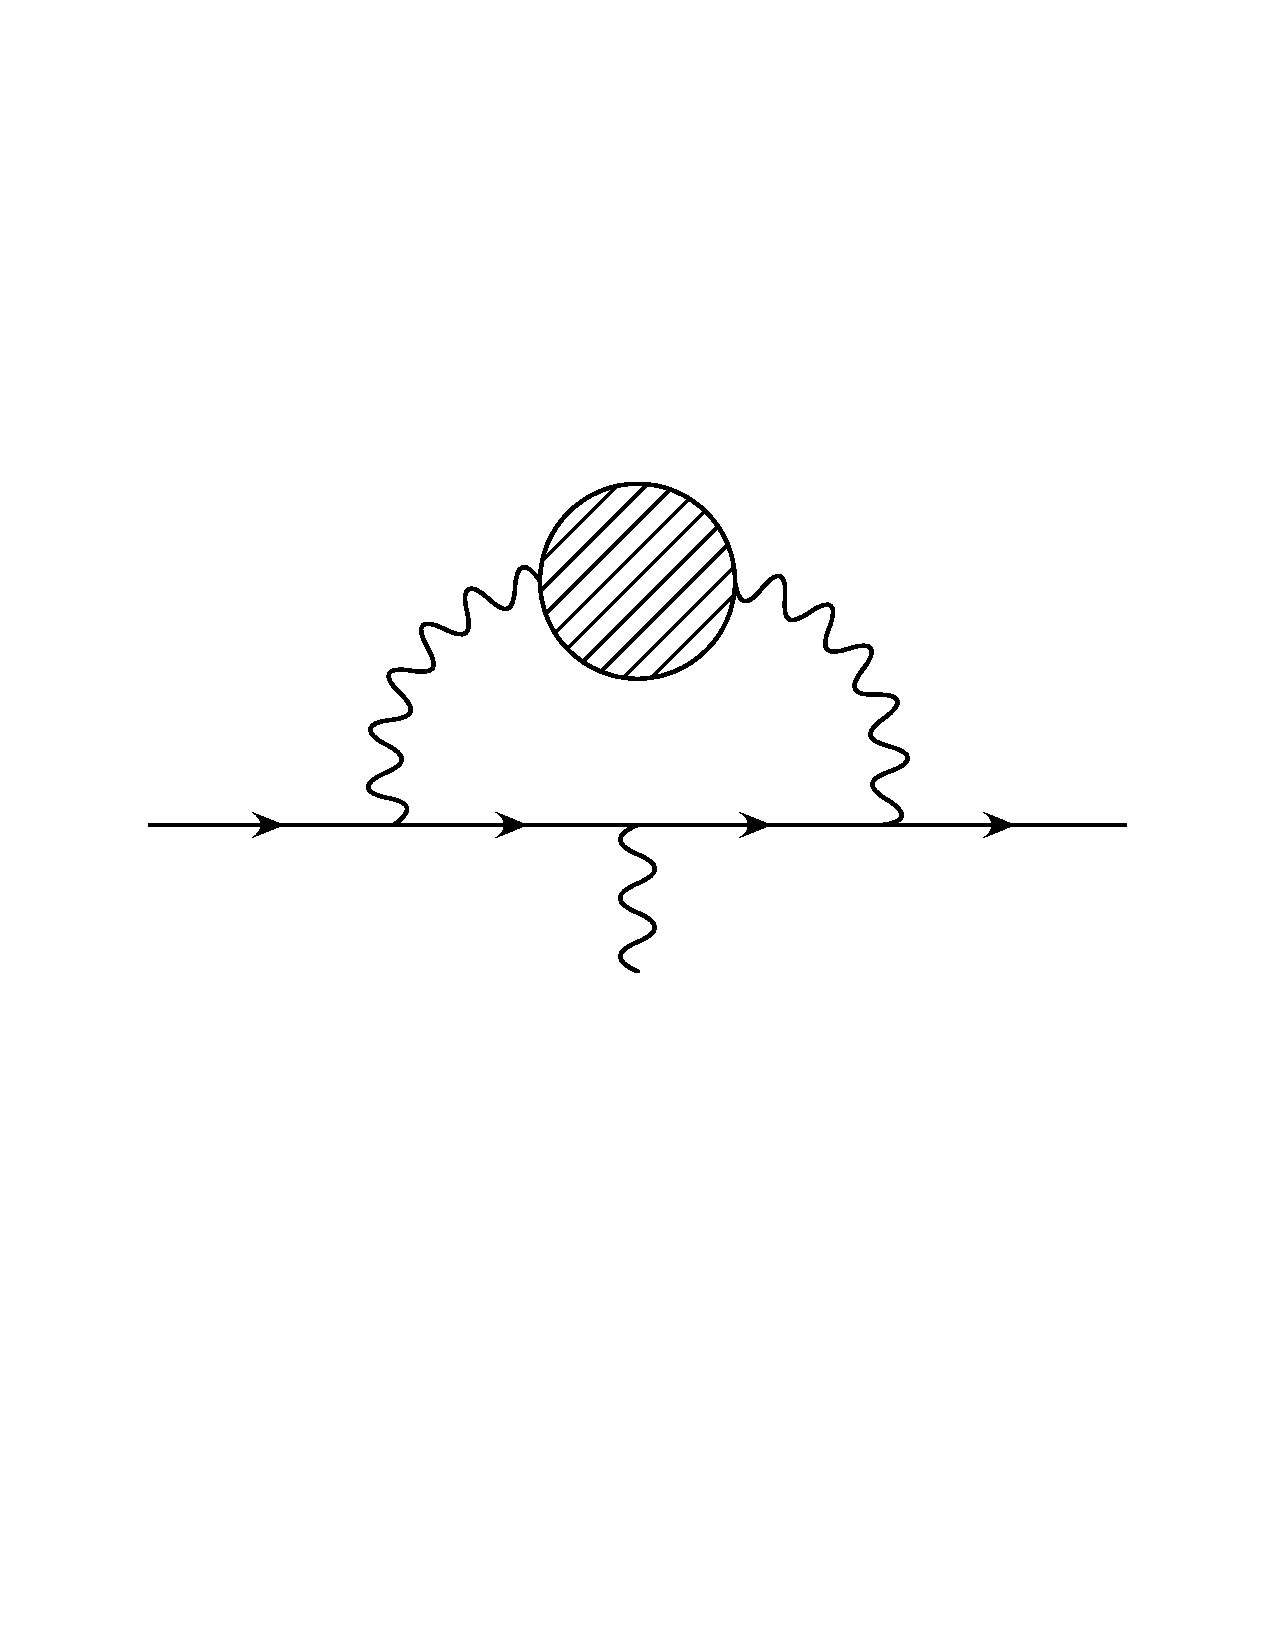
\includegraphics[width=0.3\columnwidth]{ChargedLeptons/Figures/hvp.pdf}\hskip 1cm
    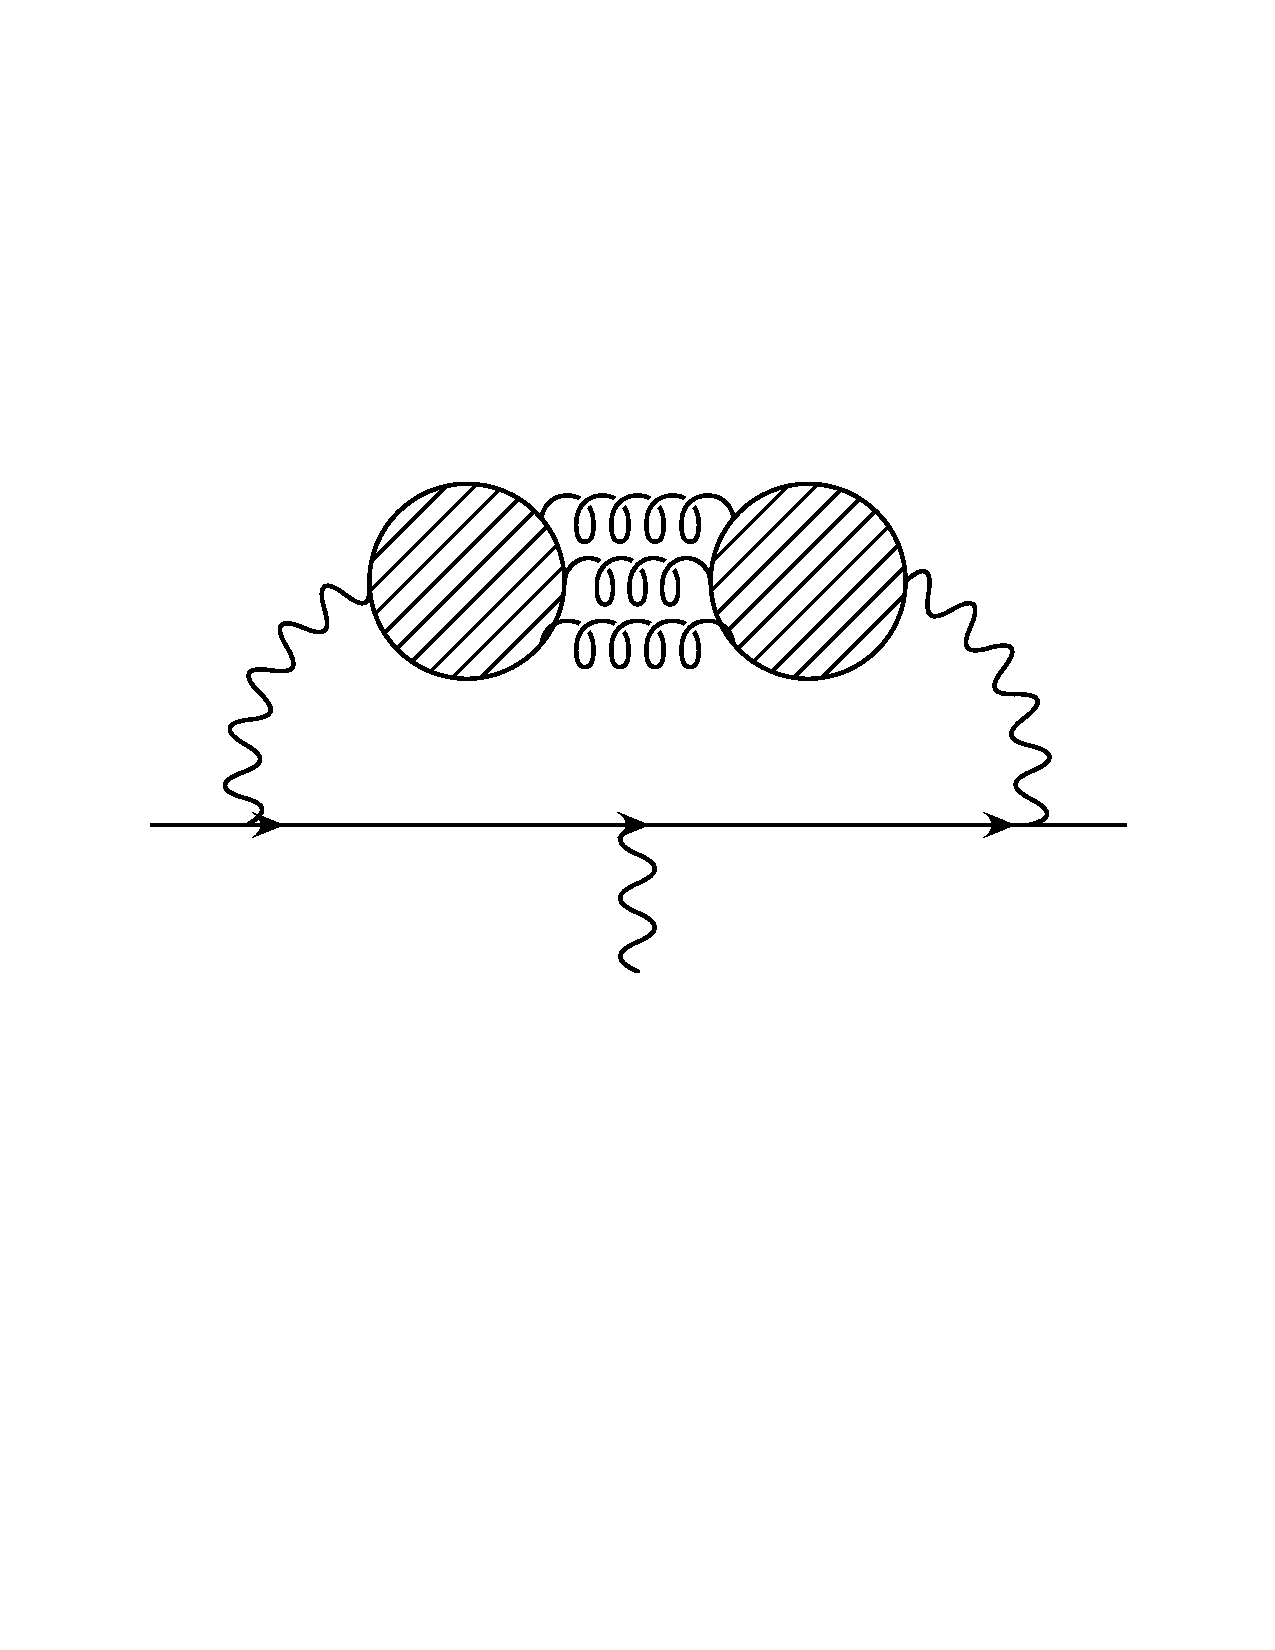
\includegraphics[width=0.3\columnwidth]{ChargedLeptons/Figures/hvp-disc.pdf}
\caption{Hadronic vacuum polarization diagrams contributing to the SM muon anomaly. The horizontal lines represent the muon. (Left panel) The blob formed by the quark-antiquark loop represents all possible hadronic intermediate states.  (Right panel) Disconnected quark line contribution. The quark loops are connected by gluons.}

    \label{fig:hvp}
\end{figure}
%

The hadronic-light-by-light (HLbL) scattering amplitude shown in
Fig.~\ref{fig:hlbl} is much more challenging.  The contribution to
$g-2$,
\begin{equation}
    a_\mu(\textrm{HLbL}) = 105(26) \times 10^{-11},
    \label{eq:PRV}
\end{equation}
is not well known. It is based on the size of various hadronic contributions estimated in
several different models~\cite{arXiv:0901.0306}.
Its uncertainty, though estimated to be less than that in a(HVP) by about 50\%, is less reliable and will be difficult to reduce with current methods.
%Its uncertainty, though less than that in $a_\mu(\textrm{HVP})$ by about a factor of two, seems harder to reduce and is expected to be the dominant uncertainty as the HVP uncertainty is reduced.
Finding a new approach, such as lattice QCD, in which uncertainties are systematically improvable,
is crucial for making greatest use of the next round of experiments.
With this in mind, a workshop was recently convened at the Institute for Nuclear Theory~\cite{INTws}.
Workshop participants discussed how models, lattice QCD, and data-driven methods could be exploited to reduce the
uncertainty on $a_\mu(\textrm{HLbL})$.
The outcome of this workshop is that 
a SM calculation of the HLbL contribution with a total uncertainty of around 10\% may be possible on the time scale of the planned experiment.
%a SM calculation of the HLbL contribution with a total
%uncertainty of 10\%, or less, can be achieved within five years. 
A detailed discussion of the computation of $a_\mu(\rm HLbL)$ in lattice QCD is given in the USQCD Collaboration white paper on $g-2$~\cite{USQCD}.
%
\begin{figure}[bp]
    \centering
\vspace*{-2pt}
    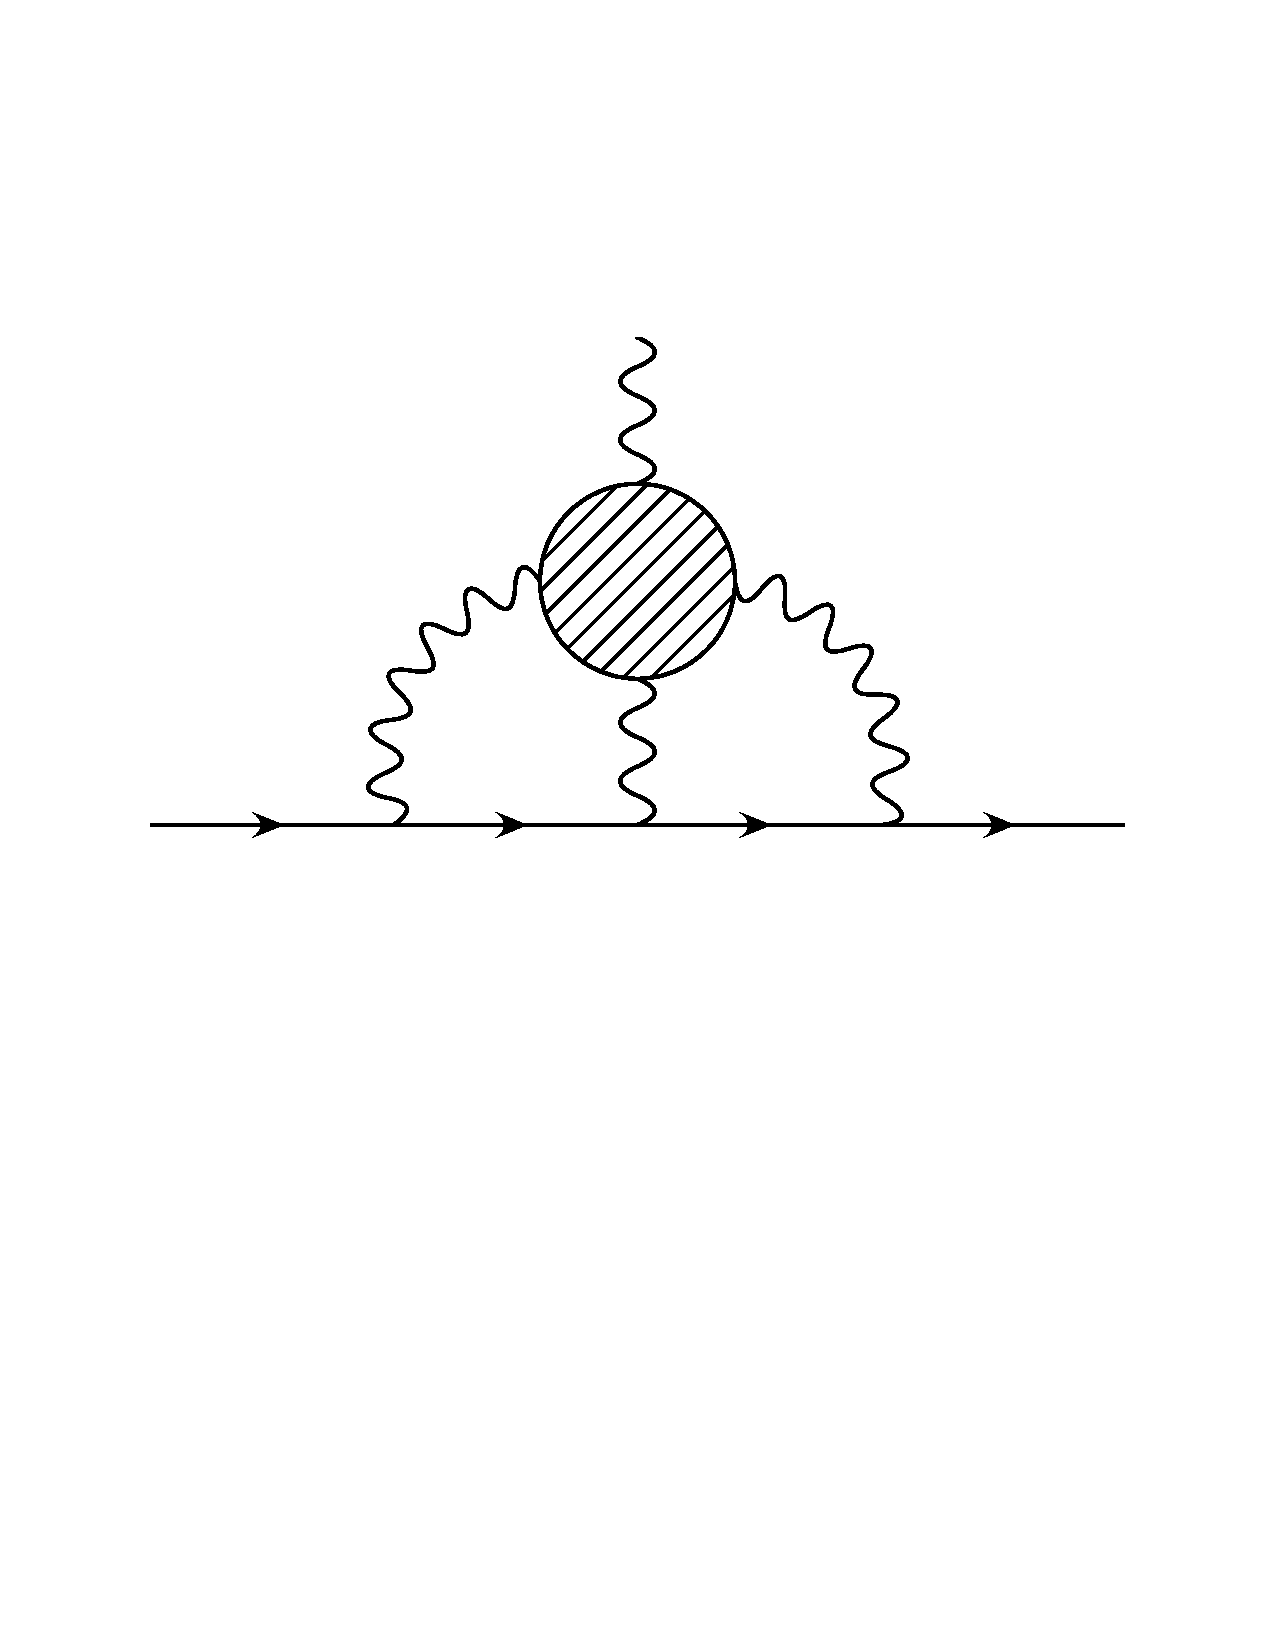
\includegraphics[width=0.3\columnwidth]{ChargedLeptons/Figures/hlbl.pdf}\hskip 1cm
    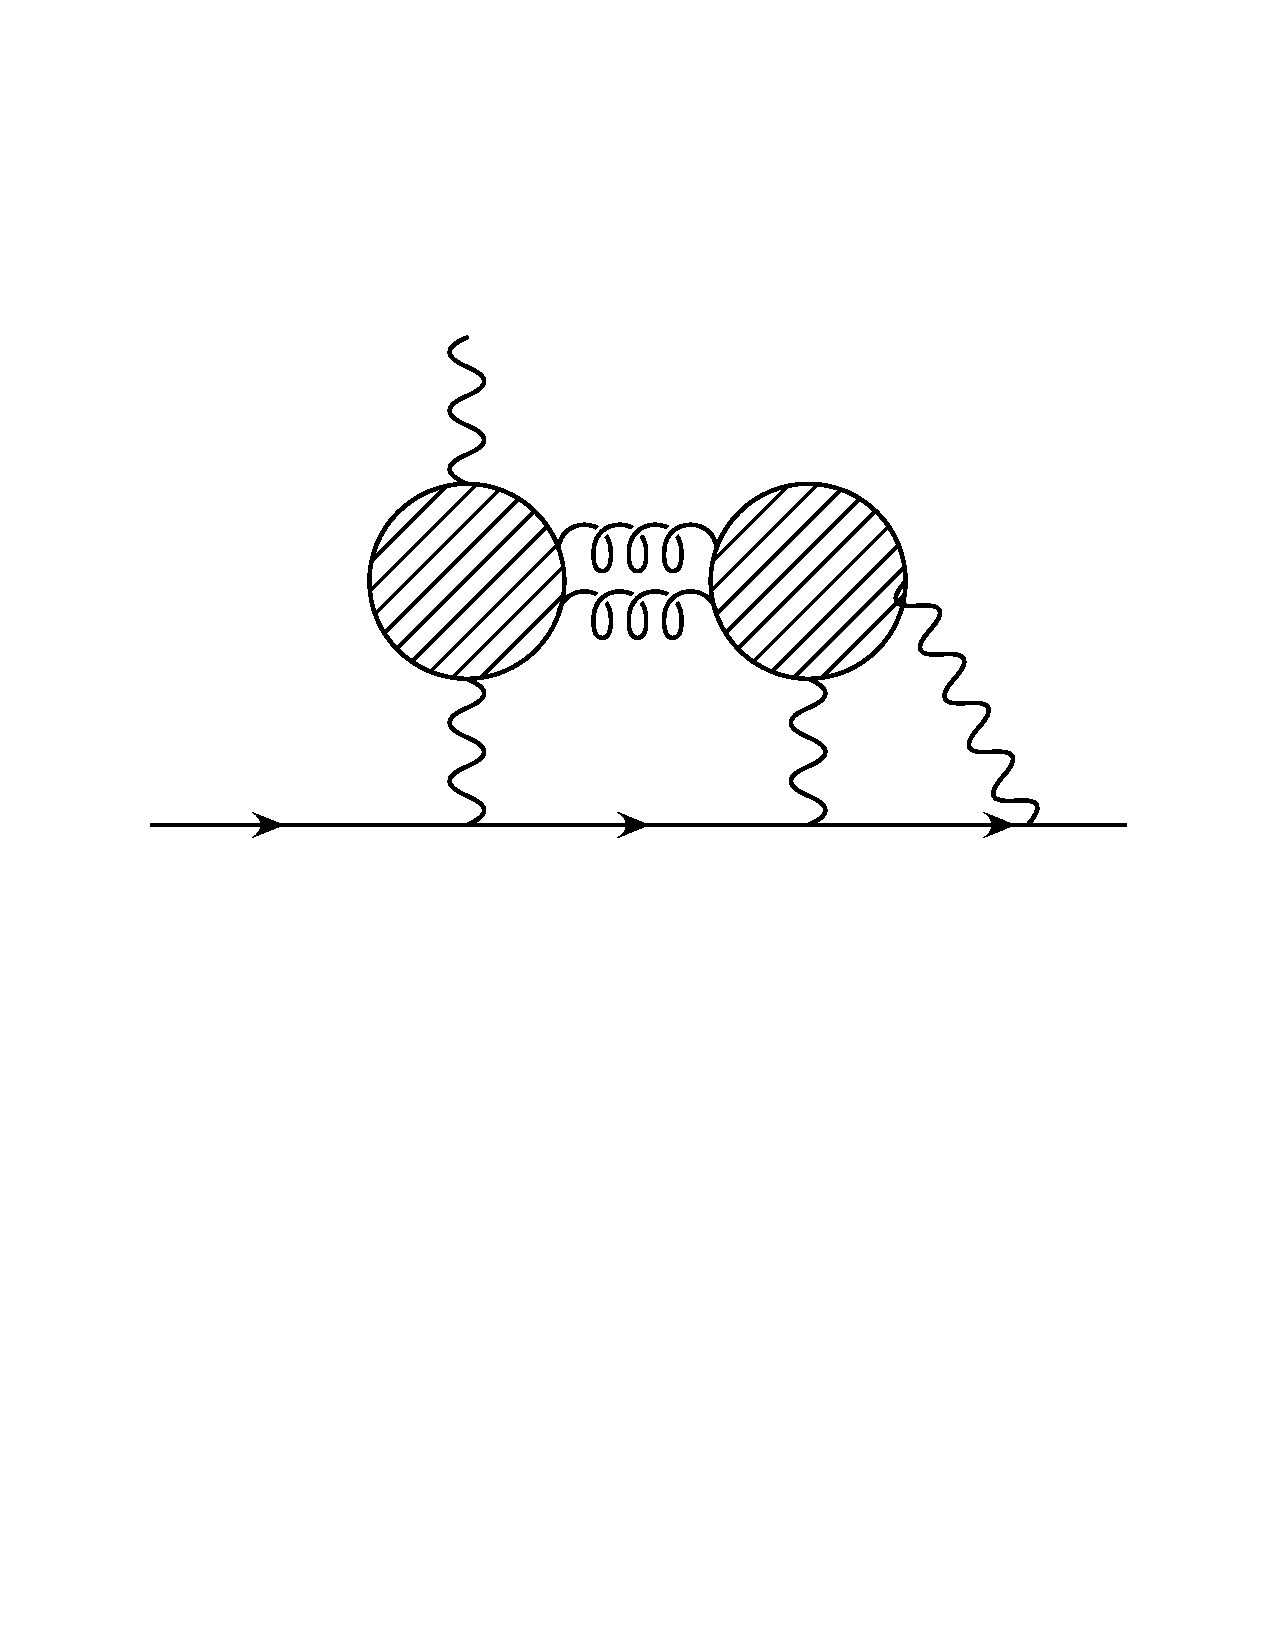
\includegraphics[width=0.3\columnwidth]{ChargedLeptons/Figures/hlbl-disc.pdf}
    \caption{Hadronic light-by-light scattering diagrams contributing to the SM muon anomaly. The horizontal lines represent the muon. (Left panel) The blob formed by the quark loop represents all possible hadronic intermediate states.  (Right panel) One of the disconnected quark line contributions. The quark loops are connected by gluons.}
    \label{fig:hlbl}
\end{figure}
%

%There are two methods, using the lattice framework, under investigation. The conventional one, analogous to the HVP calculation, is to calculate the correlation function of four electromagnetic currents for the quarks in pure QCD, one for each possible, independent, momentum configuration (there are $V^2$), fit the resulting function of discrete momenta to a smooth function and insert it into the two-loop QED integrals. The resulting four-Lorentz-index hadronic tensor has 32 independent contractions. For these reasons, the calculation is computationally demanding. An intermediate but useful step is to calculate the four-point correlation function at well chosen values of the vertex momenta to partially check model calculations.

%A second method 
The currently most promising approach using lattice methods is to compute the entire amplitude on the lattice, including the muon, in a  combined QED+QCD gauge field~\cite{hep-lat/9602005,hep-lat/0509016,827504}. The method has passed several non-trivial tests. First, it has been successfully checked against perturbation theory in pure QED. Large finite volume effects (the photons are long range) appear manageable. Preliminary calculations in full QED+QCD, at unphysical quark and muon mass and momentum transfer $q^2$, show a statistically significant result. The method requires a non-perturbative subtraction of leading order in $\alpha$ contributions which has been checked by varying the strength of the electric charge in the calculations and observing the expected scaling, before and after the subtraction. Disconnected contributions like the one shown in the right panel of Fig.~\ref{fig:hlbl} have not been included yet, but will be once the simpler first diagram (left panel, same figure) is fully under control. Calculations on a larger volume with smaller masses are in progress.

In addition to these direct approaches, there is other ongoing work on lattice-QCD calculations that check or
supplement the model calculations.
For example, it is well-known that the pion pole (namely, $\gamma\gamma^*\to\pi^0\to\gamma^*\gamma^*$)
provides the largest contribution to the QCD blob in Fig.~\ref{fig:hlbl}.
Just as experiments are being mounted to examine this physics (\emph{e.g.}, PrimEx at JLab and KLOE at LNF),
several groups~\cite{arXiv:0810.5550,arXiv:0912.0253,XFeng} are using lattice QCD to compute the amplitudes for
$\pi^0\to\gamma\gamma^*$ and $\pi^0\to\gamma^*\gamma^*$ (with one or two virtual photons).

If the SM and experiment central values do not change while both experiment and theory uncertainties are reduced, the discrepancy between the two becomes irresistible. The improvement expected from E989 (0.14 PPM) by itself improves $\Delta a_\mu$ to 5$\sigma$. A simultaneous decrease in the HLbL uncertainty to 10\% from the current 25\% pushes it to 6$\sigma$, and finally, reducing the uncertainty on the HVP contribution by a factor of two increases it to 9 $\sigma$. Such a large and clear difference between experiment and the Standard Model for the muon $g-2$ will be extremely  discriminating between new physics scenarios responsible for this discrepancy and will significantly leverage results from the energy frontier being explored at the LHC.



